% CONCLUSIONS
\chapter*{Synthèse et perspectives}
\markboth{Synthèse et perspectives}{}
\addcontentsline{toc}{chapter}{Conclusions et perspectives}
\newpage

L'étude des flux de carbone dans les écosystèmes tourbeux est complexe car assujetti à des facteurs de contrôle dont la prépondérance varie fortement selon l'échelle considérée et les conditions environnementales.
Les effets d'un facteur contrôlant sur un flux de gaz vont généralement dans le même sens dans la littérature : 
une hausse de la température à tendance à augmenter les flux.
Une augmentation du niveau de la nappe à tendance à favoriser la production de \chh par rapport à celle du \coo.
La végétation semble faciliter les échanges de gaz et libère des substrats facilement mobilisables.
Outre le fait que ces facteurs co-varient et qu'il donc difficile de distinguer leurs effets, ces effets sur les différents flux en terme de bilan de carbone est beaucoup moins nette, d'où la nécessité d'estimer des bilans de carbone sur ces écosystèmes.

\section*{Bilan du bilan (de C) ?}

Il semble cohérent que les flux de \coo de la tourbières de La Guette soit plus fort que ceux mesurés dans des tourbières boréales.
De par sa position géographique, le site à une température moyenne annuelle du site relativement élevée, et subit un climat moins dur avec des hivers moins longs et froids.
Par ailleurs il semble également cohérent que ces valeurs n'atteignent pas celles estimées dans les tourbières utilisées comme des prairie permanentes, notamment car ces dernières ont généralement un niveau le nappe d'eau plus bas.

%\boiteonglet}}

%\raisebox{1cm}[0pt][0pt]{\boiteonglet}
%\onglet


Les observations réalisées sur la tourbière de La Guette ont permis de mettre en évidence des flux de \coo particulièrement fort que ce soit pour la RE ou la PPB.
Ces flux annuels, plus fort que ceux relevés dans les tourbières boréales, sont cependant moins important que ceux mesurés dans des tourbières utilisées comme pairies permanentes.
Ces observations sont cohérentes avec les observations de terrain.
En effet la présence d'une végétation vasculaire herbacée largement dominante (\textit{Molinia caerulea}) rapproche davantage la tourbière de La Guette d'une prairie tourbeuse que d'une tourbière boréale ou prédomine les sphaignes.
Le niveau de la nappe particulièrement élevé pendant les deux années de mesure a probablement limité en partie les flux de \coo sans pour autant les empêcher.
En effet à la fois Molinia caerulea et Eriophorum Augustifolium (\textbf{Vaginatum oui mais augustifolium ?}) possèdent un aérenchyme, cette adaptation aux milieux inondés leur permettant de maintenir des échanges gazeux de leurs racines à l'atmosphère.
Par ailleurs la situation géographique locale et globale du site: une tourbière de plaine située à basse latitude, joue également sur la saisonnalité du climat, plus faible qu'en montagne, et permettant aux flux de rester plus fort pendant une période de l'année plus importante.
Les flux de \chh ne semblent quant à eux pas être contraint par le niveau de la nappe pendant les deux années de mesures.
Leur relation avec la végétation laisse encore une fois penser un effet possible de l'aérenchyme.

Ces travaux ont également montrés la forte variabilité spatiale des flux de \coo.
Le nombre limité de points de mesure du \chh ne permettant pas d'affirmer quoi que ce soit de ce côté là.
(\textbf{dvlpé var spa + vég})

%Cette force des flux de \coo est probablement liée à sa situation géographique locale et globale : une tourbière de plaine située à basse latitude et à ses problématiques de drainage et d'envahissement par une végétation vasculaire.
%Ainsi la saisonnalité plus faible qu'en montagne permet aux flux de rester fort pendant une période de l'année plus importante.
%Ces flux importants entraînent des variations forte en terme de bilan selon les méthodologies employées, il est cependant probable que la tourbière de La Guette fonctionne actuellement comme une source de carbone.

%L'estimation du bilan à l'échelle saisonnière ne permet pas de reproduire les variations journalières, l'estimation du modèle pendant les 3 jours de mesures haute fréquence réalisés en 2013 est largement supérieure aux valeurs mesurées (Figure~\ref{fig:RE1_vs_JN})

La prise en compte de la végétation reste une difficulté importante, l'observation répétée nécessitant des mesures non destructives, souvent imprécises ou très coûteuses en temps.
Paradoxalement les zones de la tourbières fonctionnant en puits de carbone sont celle ou les herbacées sont dominantes.

\subsection*{Modélisation saisonnière et mesures horaires}

Les estimations des flux de la tourbière de La Guette par les modèles du chapitre~\ref{ch:ch3} ont été calculées à l'heure.
Elles ont donc pu être comparées aux données acquises sur le même site lors d'autres expérimentations, notamment grâce à l'utilisation de méthodes de mesures identiques sur l'ensemble de ces travaux.
Ainsi si l'on compare la RE estimée à l'aide des modèles RE-1 et RE-3 (chapitre~\ref{ch:ch3}) aux données acquises à haute fréquence (chapitre~\ref{ch:ch5}) on observe un écart important entre les valeurs mesurées et celles estimées par les modèles (Figure~\ref{fig:RE1_vs_JN}).
Pour expliquer cet écart on peut considérer les deux points suivants : 

Premier point, on compare des modèles qui prennent en compte la variabilité spatiale du site (une partie au moins, à travers les vingts points qui on servi à les calibrer) à des mesures réalisées sur quatre embases dans une zone restreinte de la tourbière (20 x \SI{20}{\metre}).
Ces quatre points ayant une représentativité spatiale limitée et ont été choisi pour leur similarités.
Cet écart peut donc être en partie le reflet de la variabilité spatiale des flux dans la tourbière.
Cet argument est soutenu par les mesures de RE réalisées le 24 et le 25 juillet 2013, soit 5 jours avant les mesures haute fréquence et dont la gamme de valeur est comprise entre \num{4.8} et \SI{18.9}{\uml} et sont représentés par le fond gris sur la figure~\ref{fig:RE1_vs_JN}.
Les estimations des modèles RE-1 et RE-3 restent d'ailleurs majoritairement dans cette gamme de valeurs.
Par ailleurs, la placette p04 (Figure~\ref{fig:carteVS}) la plus proche des mesures haute fréquences, est dans la gamme basse des flux que ce soit pour la campagne du 24-25 juillet : troisième flux le plus faible mesuré (\SI{6.1}{\uml}) ou en moyenne sur l'ensemble de mesure ou elle vaut \SI{2.81(160)}{\uml} par rapport à la moyenne de l'ensemble des placettes valant \SI{3.77(289)}{\uml}.

Second point, le modèle est calibré à partir de moyennes des flux par campagne de mesure (Figure~\ref{fig:ER_evolution_avg}).
Ces moyennes sont comprises entre \num{0.69(027)} et \SI{9.43(348)}{\uml}, par conséquent les estimations des modèles, dont RE-1, en dehors de cette gamme sont du domaine de l'extrapolation et donc à considérer avec précaution.

\begin{figure}
\centering
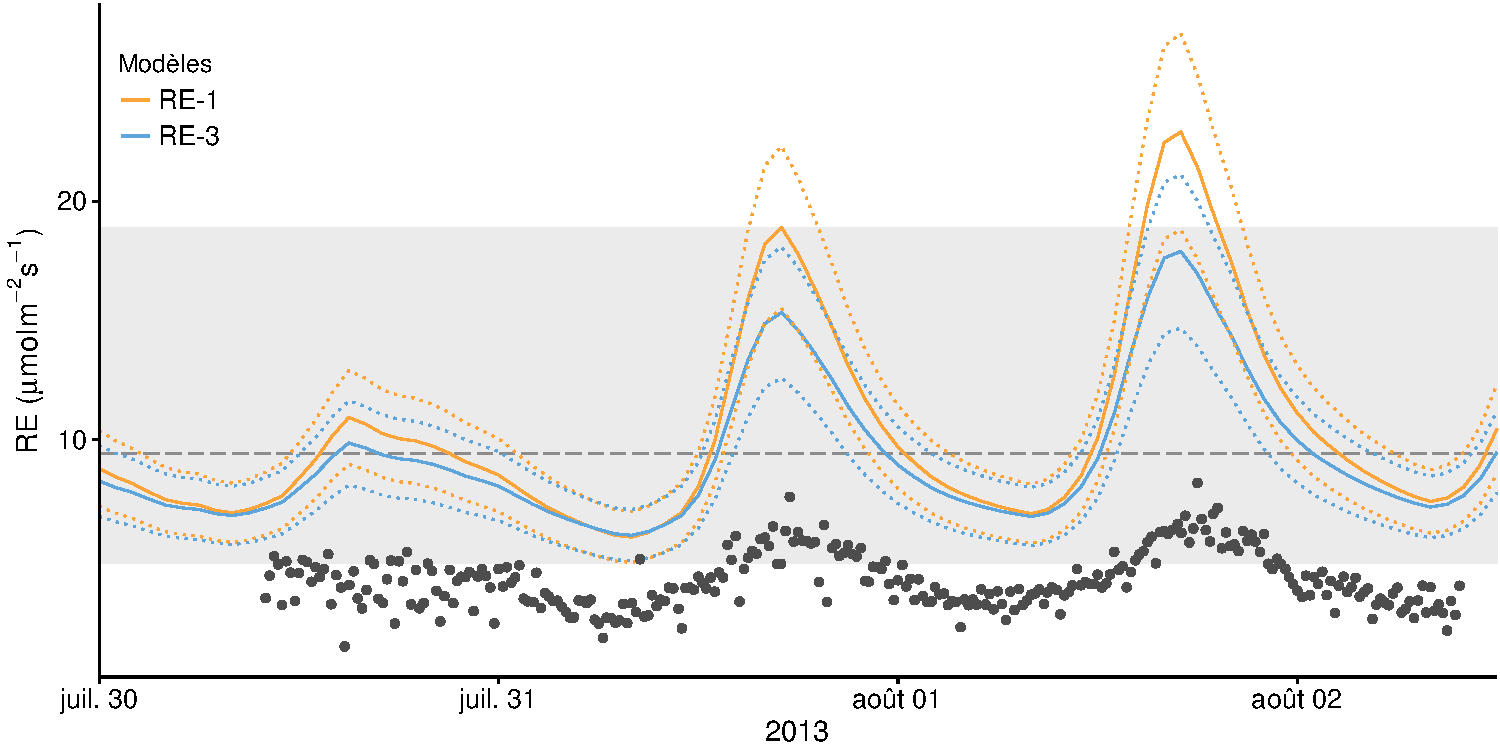
\includegraphics[width=1.15\textwidth, center]{conclusions/RE1_vs_JN}
\caption{Comparaison entre les valeurs estimées par les modèle RE-1 (ligne orange), RE-3 (ligne bleue) et les mesures faites à haute fréquence sur le site du 30 juillet au 2 août 2013 (points noirs). Les lignes de pointillés représentent l'erreur (NRMSE) associée aux modèles. La zone grisée correspond à la gamme de valeur de la RE mesurée sur l'ensemble des 20 placettes pendant la campagne du 24-25 juillet 2013. La ligne de tiret correspond à la moyenne de la RE pour cette campagne.}
\label{fig:RE1_vs_JN}
\end{figure}

Ces deux points considérés, il semble que les estimations des modèles RE-1 et RE-3, malgré les écarts que l'on peut observées, restent cohérentes avec les mesures effectuées aux différentes échelles.
Le modèle RE-3 restant davantage encore que le modèle RE-1 dans la gamme de valeur attribuable en grande partie, à la variabilité spatiale.
Cette comparaison montre également l'importance de la variabilité spatiale des flux dans les tourbières et la difficulté qu'il peut y avoir à la prendre en compte de façon satisfaisante.



\section*{L'hydrologie}

L'effet de la restauration hydrologique de la tourbière de La Guette n'a pas pu être mis en évidence de part une pluviométrie forte et un niveau de nappe toujours important.
Les expérimentations

\subsection*{Résilience de la tourbe par rapport aux 2 années sèches qui précèdent le BdC}
(lien chap 3 et 4)

%schéma conceptuel ? Modèles globaux (ORCHID, chloée)
%
%Flux fort
%
%sensibilité param forte
%
%Modèles multi annuel et prise en compte de la végétation
%
%Quid des variations journalières dans un bilan annuel ? (Figure~\ref{fig:RE1_vs_JN})


Les prendre en compte améliorerait-il les modèles

modèles globaux ?
\textbf{limitations des équations :}
Plus généralement, la majorité des tourbières sont sous la neige une partie de l'année, ce qui n'arrive que rarement sur la tourbière de La Guette et une partie possède également des zones d'eau libre, qui n'existent pas sur ce site.

modèles globaux et profondeur de tourbe


\section*{Ouverture vers d'autre méthodes de mesures}
\begin{itemize}
\item chambre automatique (lien chap 5, et chap 3 ?)
\item tour eddy covariance (lien chap 5 et chap 3 ?)
\end{itemize}

\section*{perspectives}

La suite du projet CARBIODIV permettra peut être de mettre en évidence l'effet de la restauration.

Un partenariat avec le LSCE commencé pendant ces travaux devra permettre de valoriser ces données à des échelles plus importante.
Des données on d'ors et déjà été envoyée à Chloé XX qui développe un code "tourbière" dans le modèle ORCHIDEE.

L'installation prochaine d'une tour eddy covariance sur le site permettra de comparer ce bilan à des mesures plus haute fréquence.

Modèles : PCARS (frolking2002), MWM (Wu2013), TOPMODEL (Stocker2014)


\section*{idées}

L'amélioration du protocole de végétation (RVI ?)

Amélioration des chambres (contrôle de la température ? de la vitesse du ventilateur ? plus grande ? aquisition automatisée du PAR sur la chambre)

l'inclusion des arbres

Correction du volume par pondération de la surface

Utilisation de chambres automatiques/EC

Humidité du sol

Propriétés physique de la tourbe (en cours)

